\documentclass{article}

% if you need to pass options to natbib, use, e.g.:
% \PassOptionsToPackage{numbers, compress}{natbib}
% before loading nips_2018
\usepackage{biblatex}
\addbibresource{functionalNN.bib}
\usepackage{url}
\setcounter{biburllcpenalty}{7000}
\setcounter{biburlucpenalty}{8000}


% ready for submission
\usepackage[preprint]{nips_2018}

% to compile a preprint version, e.g., for submission to arXiv, add
% add the [preprint] option:
% \usepackage[preprint]{nips_2018}

% to compile a camera-ready version, add the [final] option, e.g.:
% \usepackage[final]{nips_2018}

% to avoid loading the natbib package, add option nonatbib:
% \usepackage[nonatbib]{nips_2018}

\usepackage[utf8]{inputenc} % allow utf-8 input
\usepackage[T1]{fontenc}    % use 8-bit T1 fonts
\usepackage[linktocpage]{hyperref}       % hyperlinks
\usepackage{url}            % simple URL typesetting
\usepackage{booktabs}       % professional-quality tables
\usepackage{amsfonts}       % blackboard math symbols
\usepackage{nicefrac}       % compact symbols for 1/2, etc.
\usepackage{microtype}
\usepackage{varwidth}
\usepackage{mathtools}
\usepackage{minted}
\usepackage{algorithm}
\usepackage{csquotes}
\usepackage{enumitem}   
\usepackage{graphicx,txfonts}
\usepackage{qtree}
\usepackage{tikzsymbols} 
\usepackage{xmpmulti}% microtypography
\usepackage{hyperref}
\hypersetup{colorlinks,citecolor=red, filecolor=black, linkcolor=blue, urlcolor=black} 
\usepackage{setspace}
\DeclareMathOperator*{\argmin}{arg\, min}
\DeclareMathOperator*{\argmax}{arg\, max}
\newcommand{\norm}[1]{\left \lVert #1 \right \rVert}
\newcommand{\given}{\hspace{1mm} | \hspace{1mm}}
\newcommand{\nlim}{\underset{n}{\lim} \hspace{1mm}}
\newcommand{\bootmean}{\bar{X}_n^*}
\newcommand{\Var}{\mathbf{Var}}
\newcommand{\Exp}{\mathbf{E}}
\newcommand{\Prob}{\mathbf{P}}
\newcommand{\Cov}{\mathbf{Cov}}
\newcommand{\mb}[1]{\bs{#1}}
\newcommand{\bs}[1]{\boldsymbol{#1}}
\newcommand{\tr}{\mathrm{tr}}
\usepackage{blindtext} 
\definecolor{darkseagreen}{rgb}{0.56, 0.74, 0.56}
\usepackage{parskip}
\setlength{\parskip}{10pt}
\newlength{\tmpShadow}
\newcommand{\ourShadow}[2]{%
    \settowidth{\tmpShadow}{#1}
    \addtolength{\tmpShadow}{.1em}
    \raisebox{-0.25ex}{\textcolor{gray!70}{#1}}%
    \kern-\tmpShadow%
    \textcolor{#2}{#1}%
}

%\renewcommand\footnoterule{{\color{black}\hrule height 0.5pt}} 

\newcommand{\heart}{\ensuremath\varheartsuit}
\newcommand{\butt}{\rotatebox[origin=c]{180}{\heart}}

\usepackage[noend]{algpseudocode}
\makeatletter
\def\BState{\State\hskip-\ALG@thistlm}
\makeatother
\vspace{10em}
\usepackage{tcolorbox}
\usepackage{etoolbox}
\BeforeBeginEnvironment{minted}{\begin{tcolorbox}}%
\AfterEndEnvironment{minted}{\end{tcolorbox}}%
\usepackage{listings}

\lstset{ 
  language=R,                     % the language of the code
  basicstyle=\small\ttfamily, % the size of the fonts that are used for the code
  numbers=left,                   % where to put the line-numbers
  numberstyle=\tiny\color{Blue},  % the style that is used for the line-numbers
  stepnumber=1,                   % the step between two line-numbers. If it is 1, each line
                                  % will be numbered
  numbersep=5pt,                  % how far the line-numbers are from the code
  backgroundcolor=\color{white},  % choose the background color. You must add \usepackage{color}
  showspaces=false,               % show spaces adding particular underscores
  showstringspaces=false,         % underline spaces within strings
  showtabs=false,                 % show tabs within strings adding particular underscores
  frame=single,                   % adds a frame around the code
  rulecolor=\color{black},        % if not set, the frame-color may be changed on line-breaks within not-black text (e.g. commens (green here))
  tabsize=2,                      % sets default tabsize to 2 spaces
  captionpos=b,                   % sets the caption-position to bottom
  breaklines=true,                % sets automatic line breaking
  breakatwhitespace=false,        % sets if automatic breaks should only happen at whitespace
  keywordstyle=\color{RoyalBlue},      % keyword style
  commentstyle=\color{YellowGreen},   % comment style
  stringstyle=\color{ForestGreen}      % string literal style
}

\title{Functional Neural Networks}

% The \author macro works with any number of authors. There are two
% commands used to separate the names and addresses of multiple
% authors: \And and \AND.
%
% Using \And between authors leaves it to LaTeX to determine where to
% break the lines. Using \AND forces a line break at that point. So,
% if LaTeX puts 3 of 4 authors names on the first line, and the last
% on the second line, try using \AND instead of \And before the third
% author name.

\author{
  Barinder Thind\thanks{\url{https://b-thi.github.io}} \\
  Department of Statistics \& Actuarial Science\\
  Simon Fraser University\\
  Burnaby, British Columbia\\
  \texttt{bthind@sfu.ca} \\
  %% examples of more authors
  %% \And
  %% Coauthor \\
  %% Affiliation \\
  %% Address \\
  %% \texttt{email} \\
  %% \AND
  %% Coauthor \\
  %% Affiliation \\
  %% Address \\
  %% \texttt{email} \\
  %% \And
  %% Coauthor \\
  %% Affiliation \\
  %% Address \\
  %% \texttt{email} \\
  %% \And
  %% Coauthor \\
  %% Affiliation \\
  %% Address \\
  %% \texttt{email} \\
}
\usepackage[10pt]{extsizes}
\begin{document}
% \nipsfinalcopy is no longer used
\vspace{10em}
\maketitle

\begin{abstract}
\doublespacing
\noindent Neural networks have shown to be an extraordinarily powerful methodology in the the realm of multivariate analysis. For example, \textit{resnet50}, a Google trained residual neural network \cite{resnet} has remarkable accuracy when attempting to classify over 150 household items. However, these methods have been limited to discrete inputs; functional data analysis \cite{fda} is a branch of statistics that re-imagines how we view information - letting observations be infinitely dimensional, we can apply operations that would otherwise seem unreasonable (for example, taking a derivative of an observation). This paper extends neural networks to the functional space through a reformulation of the activations on which the neural network optimizes. In particular, a family of networks are introduced for scalar responses with functional covariates. The groundwork is placated for functional responses in both the context of functional covariates and scalar covariates. The family of methodologies introduced here includes feed-forward neural networks, residual neural networks, recurrent neural networks, and neural ordinary differential equations. Moreover, an \textbf{R} package, developed on top of \textit{keras} will be made available for implementation of this approach.\\

\noindent \textbf{Keywords:} Functional Data, Neural Networks, Gaussian Quadrature, Residual Networks, Functional Linear Models

\end{abstract}
\newpage
\tableofcontents

\newpage
\section{Introduction}
\label{section:one}

\noindent The ever-expanding umbrella that encompasses deep-learning methodologies has been limited to the multivariate scope. With the advent of and rise of functional data analysis (FDA) \cite{fda}, it is natural to extend neural networks to this (functional) space. More specifically, this paper introduces functional feed-forward neural networks, functional residual neural networks, and functional neural ordinary differential equation networks.

\noindent In \hyperref[section:functionalNetworks]{Section II}, functional neural networks are introduced. The family of nine networks are presented along with their mathematical details and some empirical results highlighting their use. In the \hyperref[sec:appendix]{Appendix}, functional data is presented with some\textit{depth} regarding this sub-domain of statistics including the introduction of functional linear models - a methodology that is highly pertinent to understanding the general functional neural network. Also in the \hyperref[sec:nn]{Appendix}, feed-forward, residual, and neural ordinary differential equations are outlined with varying degrees of information. Moreover, there is a \hyperref[sec:de]{subsection} presented on differential equations that provides the relevant details in understanding subsequent sections. All code will be provided in a separate \textit{.rmd} file and is also available in the appendix. Note, the family of networks introduced here will be incomplete at the time of submission of this project - the hope is that there is enough motivation to continue and develop on the ideas here further.

\section{Functional Neural Networks}
\label{section:functionalNetworks}
\vspace{-7pt}
\begin{figure}[h!]
  \centering
  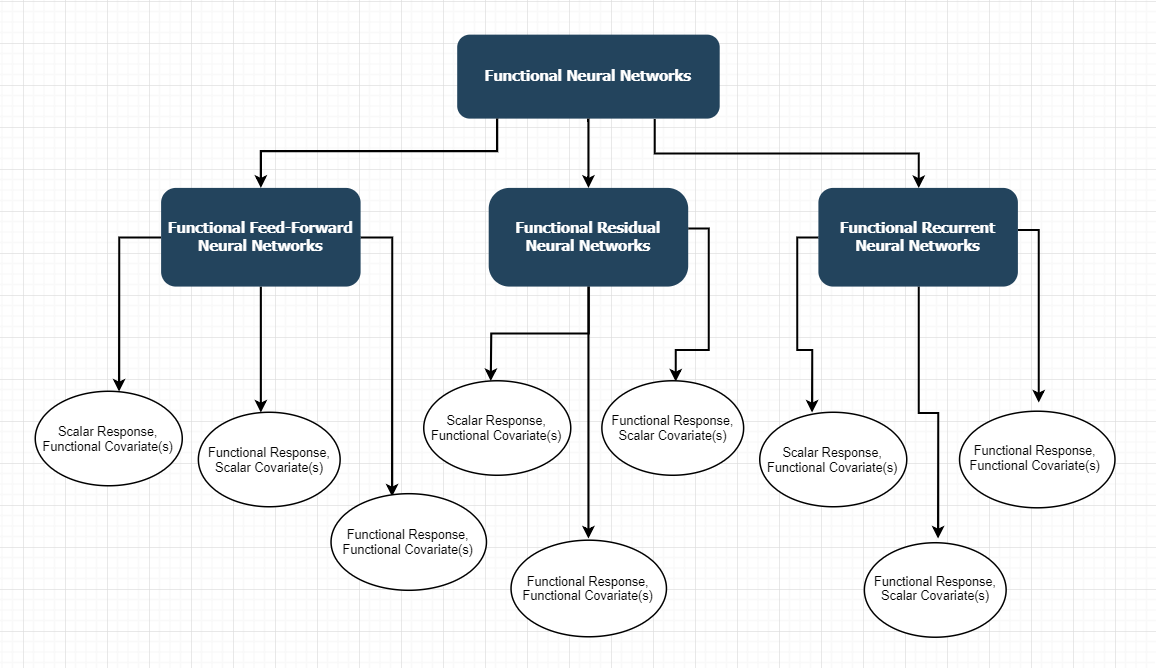
\includegraphics[scale = 0.6]{overview.png}
  \label{fig:family}
  \caption{An overview of the family of neural networks introduced in this paper}
\end{figure}
\vspace{-7pt}
\noindent In this section, functional neural networks are introduced in the context of feed-forward, residual, and recurrent neural networks for a scalar response and functional covariate. Then, groundwork is laid for the other two types of functional linear models. The general umbrella of this family of new neural networks can be seen in \hyperref[fig:family]{Figure 1}. Any jargon or gaps in knowledge can potentially be remedied by the fairly exhaustive \hyperref[sec:appendix]{Appendix.}

\subsection{Functional Feed-Forward Networks}
\label{sec:funcFeedNN}

\subsubsection{Forward Pass: Scalar Response, Functional Covariate(s)}

In \hyperref[sec:nn]{6.2.1}, it is shown that a neural networks largely take roles as function approximators and, in fact, they themselves are a kind of recursive function. For example, consider a network that takes a 1 dimensional input, has 2 hidden layers, and outputs a 1 dimensional scalar value. Then the entire neural network can be written as:
\begin{align}
    \hat{y} = \underbrace{\sigma(w_{3}\cdot[\underbrace{\sigma(w_{2}(\underbrace{\sigma(w_{1}x_{1} + b_{1})}_\text{$z^{(1)}_{1}$}) + b_{2})}_\text{$z^{(2)}_{1}$}] + b_{3})}_\text{$z^{(3)}_{1} = \hat{y}$}
\end{align}

\noindent Where $\sigma(.)$ is some activation function, $w = \{w_{1}, w_{2}\}$ is the vector of weights\footnote{In this 1 dimensional case}, and $b$ is the bias. The functional form of this model can be rewritten as:
\begin{align}
    \hat{y} = \underbrace{\sigma(w_{3}\cdot[\underbrace{\sigma(w_{2}(\underbrace{\sigma(\int w_{1}(t)x_{1}(t)dt + b_{1})}_\text{$z^{(1)}_{1}$}) + b_{2})}_\text{$z^{(2)}_{1}$}] + b_{3})}_\text{$z^{(3)}_{1} = \hat{y}$}
\end{align}

\noindent To make this more clear, let's take a step back in the process and consider the input neuron: $x$. In the usual case, this will be exactly a single observation with one co-variate. In the functional analogue here, this relates to a functional observation pre-defined as a linear combination of basis functions. Since the case(s) thus far have been limited to a scalar response, we can be content knowing that the transformation of the functional observation $x(t)$ is a scalar as it enters the exits out of the first hidden layer\footnote{That is, $z^{(1)}$ is a scalar}. The rest of the network flows as in the usual case.


\noindent In order to move forward here, an integral approximation is required. The approximation technique of choice used here is \textit{Gaussian Quadrature}; this algorithm is specifically useful for polynomial functions \cite{quad4} \cite{quad3} and since we will be defining many of the basis with b-splines\footnote{See the \hyperref[sec:appendix]{Appendix}}, this is an optimal choice\footnote{Gaussian Quadrature tends to perform extremely well on polynomial approximation problems}. The trapezoidal rule requires equally spaced notes in some interval, $[a, b]$ however Gaussian Quadrature relaxes this assumption.

\begin{figure}[h!]
  \centering
  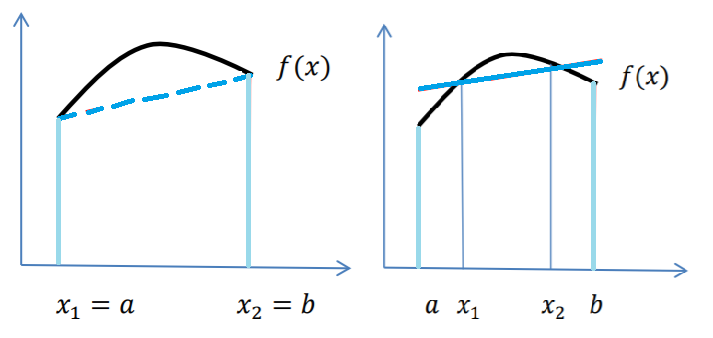
\includegraphics[scale = 0.75]{comp_integ.png}
  \label{fig:mapped}
  \caption{On the left, we see an illustration of the Trapezoid rule for numeric integration approximation and, on the left, we see the Gaussian Quadrature approach \cite{quad}}
\end{figure}

\noindent As an aside, the paper uses Gaussian Quadrature based on Legendre polynomials - the integration points are the roots of these polynomials. The approach gives an exact answer if the function, $f(x)$ to be approximated is a polynomial of order $2\cdot n - 1$ where $n$ is equal to the number of nodes (integration points). Also, note that Legendre polynomials are defined in the set $\{x: -1 \leq x \leq 1\}$ so the range of the function needs to be adjusted.

\begin{figure}[h!]
  \centering
  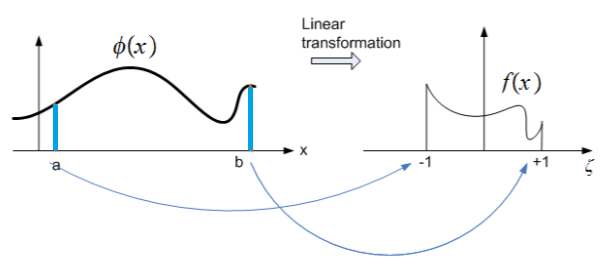
\includegraphics[scale = 0.85]{legendre.png}
  \label{fig:comp_integ}
  \caption{An illustration of the required mapping onto the new domain \cite{quad2}}
\end{figure}

\noindent Furthermore, for consistency with the book from which this information is obtained \cite{numeric_book}, let $\phi(x)$ be the function to be approximated and $f(x)$ be the mapped function; this can be seen in \hyperref[fig:mapped]{Figure 3}. The algorithm then is outlined as follows:

\begin{algorithm}[H]
\caption{Guassian Quadrature}\label{alg:quad}
\begin{algorithmic}[1]
\Statex \textbf{Input}: $\phi(x), a, b$
\Statex \textbf{Output}: A numerical value for $\int_{a}^{b}\phi(x)dx$ 
\State Specify some value $n$ for the number of nodes to be evaluated within the range $[a, b]$
\State Use the look up table (done automatically in progamming languages) to find a set of weights, $\alpha_{i}$ for the integration points $x_i$
\State Initiate: Integral = 0
\Statex \hspace{1em} For $i$ in 1:$n$: Integral = Integral + \textit{GuassianQuadrature}($i$)
\Statex End;

\end{algorithmic}
\end{algorithm}

\noindent Where:
\begin{align}
GaussianQuadrature(i) = \alpha_{i}\Bigg[\dfrac{b - a}{2} \phi\Bigg(\dfrac{(b - a)x_{i}}{2} + \dfrac{a + b}{2}\Bigg)\Bigg]
\end{align}
\noindent The motivation for why we need this numerical approximation can be found in $z_{1}^{(1)}$ in (2). Examining it closer and expanding the basis from which it is formed, we find the following:
\begin{align}
    z_{1}^{(1)} &= \sigma(\int w_{1}(t)x_{1}(t)dt + b_{1})\\
    &= \sigma(\int \sum c_{i}\psi(t)x_{1}(t)dt + b_{1})\\
    &= \sigma(\sum c_{i}\underbrace{\int\psi(t)x_{1}(t)dt}_{Approximated} + b_{1})
\end{align}
\noindent The $\psi(t)$ vector is the evaluations of the basis functions of the coefficient function in the linear model at times $t$. The $x(t)$ is the functional observation. Since it is likely that no closed form or simple integral of this form will exist, Gaussian Quadrature will be used instead to estimate what this will evaluate out to. 

\noindent Now that we have a way to evaluate this integral, we can note that we have now transformed the problem from the one requiring the following derivatives:
\[\nabla R = \Bigg( \begin{array}{cc}

\dfrac{\partial R}{\partial w_{1}(t)} \ \ \
\dfrac{\partial R}{\partial w_{2}} \ \ \
\dfrac{\partial R}{\partial w_{3}} \ \ \
\dfrac{\partial R}{\partial b_{1}} \ \ \ 
\dfrac{\partial R}{\partial b_{2}} \ \ \
\dfrac{\partial R}{\partial b_{3}}
\end{array} \Bigg)^{T}\] 

\noindent To the following gradient:
\[\nabla R = \Bigg( \begin{array}{cc}

\dfrac{\partial R}{\partial c_{1}} \ \ \
\dfrac{\partial R}{\partial c_{2}} \ \ \ 
... \ \ \ 
\dfrac{\partial R}{\partial c_{k}} \ \ \
\dfrac{\partial R}{\partial w_{2}} \ \ \
\dfrac{\partial R}{\partial w_{3}} \ \ \
\dfrac{\partial R}{\partial b_{1}} \ \ \ 
\dfrac{\partial R}{\partial b_{2}} \ \ \
\dfrac{\partial R}{\partial b_{3}}
\end{array} \Bigg)^{T}\]
\noindent Where $k$ is the number of basis functions used in the formulation of the coefficient function and $R$ is the loss function\footnote{More information available in the \hyperref[sec:nn]{Appendix}}. While we increased the number of derivatives, we also decreased the computational time as the calculation of a derivative with respect to a function will result in a greater number of flops, potentially. This needs to be explored further however and there does seem to be literature which could be useful to compute that functional gradient in one swoop rather than in the descritized way it is now - this alternative approach is explored in greater detail within \hyperref[sec:backpropResFuncNN]{2.2.2}. 

\noindent At this point, we have enough information to complete the forward pass. The next section details how the model "learns".

\subsubsection{Backpropagation: Scalar Response, Functional Covariate(s)}

\noindent In the backward pass, the transformation made in (6) allows the gradient to be computed exactly as you would in a feed-forward neural network. The following algorithm describes the process:
\begin{algorithm}[H]
\caption{Backward Pass - Functional Feed-Forward Neural Network}\label{alg:backwardfuncnn}
\begin{algorithmic}[1]
\Statex \textbf{Input}: $\Hat{y}, \theta$, $j$. $i = 0$
\Statex \textbf{Output}: Updated values for the set of parameters $\theta$
\State While $j > i$:
\State Select a subset number, $f$ of observations for which the neural network is run - a mini batch
\State Compute the gradient, $\nabla R$ for each observation and normalize
\State Take the average of the corresponding gradient values across all the observations
\State Add the average, weighted by some learning rate $\gamma$ to the current values of the weights: $w_i = w_i + \dfrac{\partial R}{\partial _{w_i}}\cdot\gamma$ where $w_i$ is some parameter of the network, $\hat{y}$
\State $i = i + 1$
\State Go back to 1
\end{algorithmic}
\end{algorithm}
\noindent Note that, in step 3, the following equation might be illuminating:
\begin{align}
 \dfrac{\partial R}{\partial w_i} = \dfrac{1}{n}\sum_{i = 0}^{f - 1}\dfrac{\partial R_i}{\partial w_i} 
\end{align}
\noindent For some weight, $w_i$. This process repeats for some number of epochs - here, this was denoted by the $j$. An epoch is a full run of your observations specified before the model is run. The final model is the last set of remaining weights and biases, $\theta$ after all the updates have been applied through the iterations. The dynamic variable here, with respect to prediction, is the functional input $x(t)$.

\subsubsection{An Example: Scalar Response, Functional Covariate(s)}

\noindent In this section, an example is provided to show the predictive power of this algorithm. The data set used has information regarding the mean amount of precipitation in a year and the daily temperature for 35 Canadian cities. The functional observations are the temperature for which there are 365 (daily) time points. In total, there are 35 functional observations and the scalar response is the average precipitation. Note: there is only 1 covariate here and it is of a functional nature. The results will be compared with prediction accuracy from a functional regression model. 

\noindent Also, as a quick aside, in the computation portion here, \textit{Simpson's Composite Rule} was used for the integral approximation. This is purely due to a time constraint and the approach will revert back to \textit{Gaussian Quadrature} as time allows \cite{simpsons}.

\noindent First, we define the functional observations. For this, a Fourier basis expansion was using with 65 basis functions defining each of the 35 cities. The coefficient function of the regression model defining $z^{(1)}_{1}$ is defined using 11 basis coefficients. In total, there was 14\footnote{11 from $w_{1}(t)$, and 1 each for $w_{2}, b_{1},$ and $b_{2}$} derivatives to be computed in this neural network per backward pass. There are also 11 integral approximations computed per forward pass. A various number of epochs were computed in an attempt to minimize overfitting and it seems that the choice of 10 full passes of the data set was optimal.

\begin{figure}[h!]
  \centering
  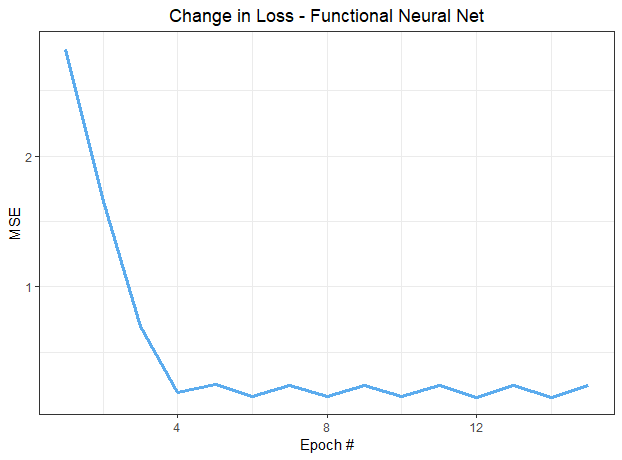
\includegraphics[scale = 0.5]{funcNNLoss.png}
  \label{fig:funcNNLoss1}
  \caption{Loss plot using 15 epochs with a learning rate of 0.1}
\end{figure}

\noindent In \hyperref[fig:funcNNLoss1]{Figure 4}, notice the oscillating behaviour from epoch 4 to epoch 15. This behaviour is characterized by a high learning rate; the derivative update seems to make too big of a leap towards the local optimum and hence, never gets closer to the optimum (as the next update shifts the final output too much in the other direction) \cite{learnRate}. This problem was circumvented using an adaptive learning rate \cite{adam}; that is, the learning rate $\gamma$, adjusts as we move through the epochs to avoid the aforementioned behaviour.

\begin{figure}[h!]
  \centering
  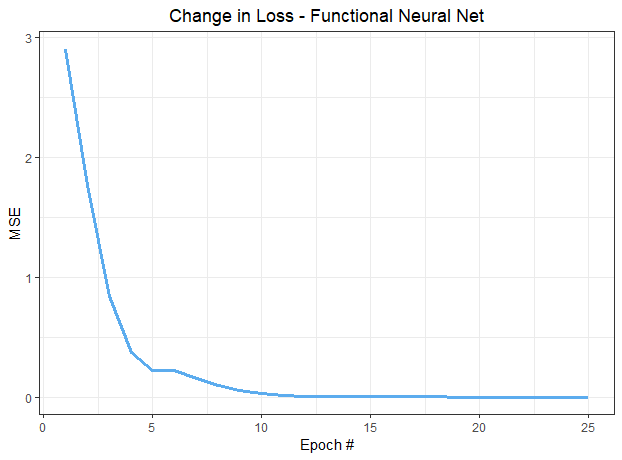
\includegraphics[scale = 0.5]{lossplot2.png}
  \label{fig:funcNNLoss2}
  \caption{Loss plot using 25 epochs with an adaptive learning rate}
\end{figure}

\noindent The functional regression model was fit as would be expected and the mean squared error values for both of these fits is given in \hyperref[table:one]{Table 1}. The loss was considerably lower in the functional neural network when compared with the functional regression model.
\begin{center}
\label{table:one}
 \begin{tabular}{||c c||} 
 \hline
 Functional Regression & Functional Neural Network \\ [1ex] 
 \hline\hline
 0.484 & 0.0304 \\ [1ex] 
 \hline
\end{tabular}\\ \smallskip
Table 1: Mean squared error values for the two different models
\end{center}

\noindent Moreover, we can even consider the differences in the $\beta$ coefficient function values. A key innovation in the functional neural network that is not available in the ordinary functional neural network is the move away from the "black-box" nature of these types of models. That is, since a leading contributor to the black-box label of neural networks is the inordinate amount of changing numbers, it can be illuminating to consider rather a function defined by these seemingly uninterpretable numbers. Remember that in the functional neural network, one of the (set of) weights we are estimating define a basis function. This basis function is extremely similar (in the 1 neuron case) to the one predicted in the functional regression model. Essentially, the final set of weights here define the 11-basis $\beta$ coefficient function and this can be compared with the usual one pulled from a function linear model.

\begin{figure}[h!]
  \centering
  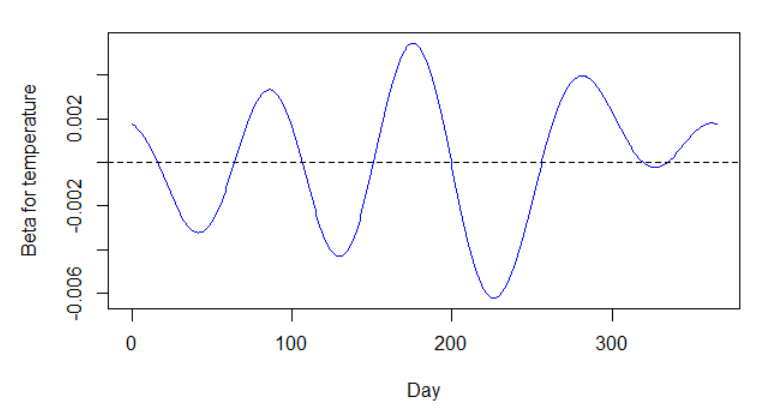
\includegraphics[scale = 0.36]{freg_beta_plot.png}
  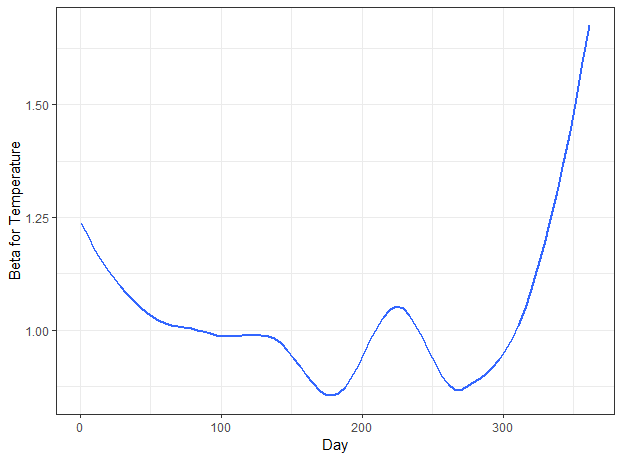
\includegraphics[scale = 0.37]{beta_coef_plot2.png}
  \label{fig:comp_betas}
  \caption{A comparison of the $\beta$ coefficient functions. It seems that there is a difference here in that the functional neural network coefficient function states that there is an increased effect of temperature around the summer of summer on mean precipitation vs. the functional regression. Moreover, there seems to be more of a disparity between the effects over time in the functional neural network when compared with the more cyclical nature of the $\beta$ coefficient function in the regression}
\end{figure}

\noindent Predictions were made on the functional observation of \textit{Resolute} to see how the models performed on a new observation, outside of the data set \cite{fda_pred}. The results are given in \hyperref[table:two]{Table 2}. 
\begin{center}
\label{table:two}
 \begin{tabular}{||c c||} 
 \hline
 Functional Regression & Functional Neural Network \\ [1ex] 
 \hline\hline
 0.242 & 6.25e-05 \\ [1ex] 
 \hline
\end{tabular}\\ \smallskip
Table 2: Resolute prediction squared errors
\end{center}

\noindent Next, we can consider the $y$ v. $\hat{y}$ and residual plots for the functional neural network given in \hyperref[fig:resPlotss]{Figure 7} and \hyperref[fig:fitted]{Figure 8}. We aren't specifically concerned with the residual plot although it is nice given the interpretable nature of this functional neural network. The other plot shows a nearly perfect linear fit.

\begin{figure}[h!]
  \centering
  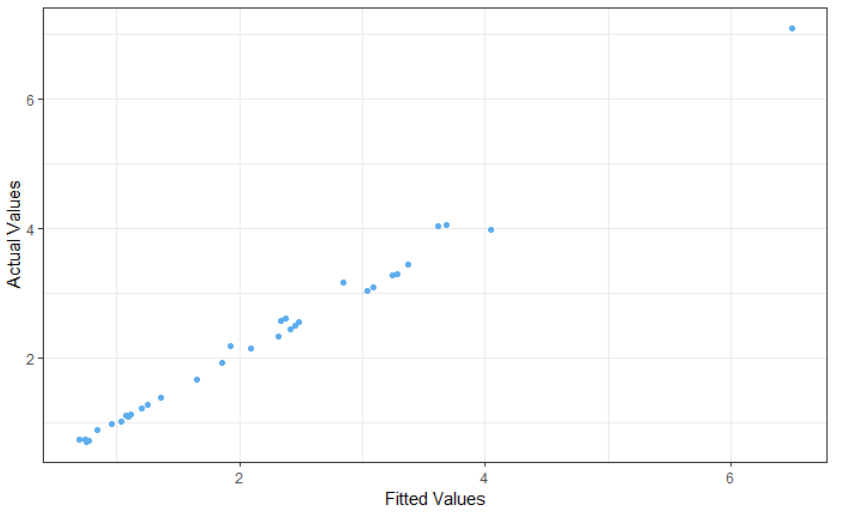
\includegraphics[scale = 0.4]{fittedvsactual.png}
  \label{fig:resPlotss}
  \caption{$y$ vs. $\hat{y}$ plot for the functional neural network}
\end{figure}

\begin{figure}[h!]
  \centering
  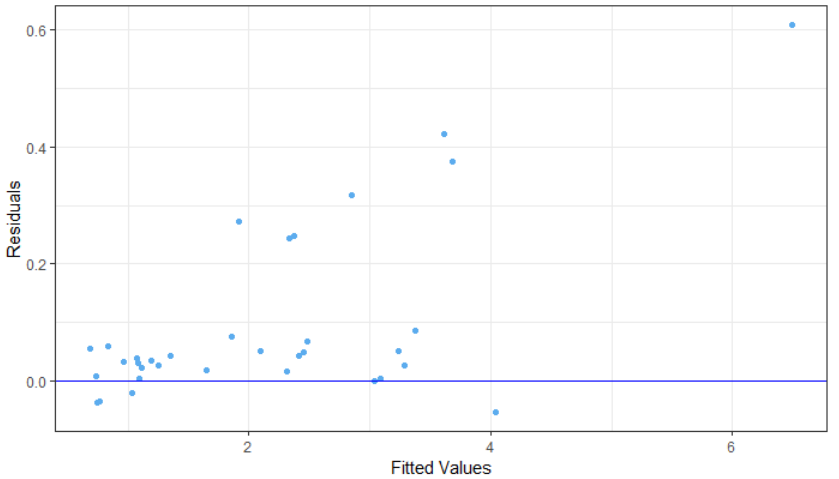
\includegraphics[scale = 0.4]{resplot2.png}
  \label{fig:fitted}
  \caption{Residual plot for the functional neural network}
\end{figure}

\noindent Next, a comparison was made between a functional neural network and regular feed-forward neural network \cite{nnInR}. In the latter case, there were 365 covariates - each corresponding to the daily temperature for the given city. The same conditions were given as in the functional case and the functional neural network outperformed its multivariate counterpart\footnote{Note, for some reason, the \textit{neuralnet} package in \textbf{R} gives varying errors so in the markdown output, the value may be different. Regardless, no amount of this variability resulted in a lower error rate than the functional neural network}:
\begin{center}
\label{table:three}
 \begin{tabular}{||c c||} 
 \hline
 Neural Network & Functional Neural Network \\ [1ex] 
 \hline\hline
 0.173 & 0.0304 \\ [1ex] 
 \hline
\end{tabular}\\ \smallskip
Table 3: Neural Network Comparison
\end{center}



\subsubsection{Current Status:}

\noindent The other variations of this type of network, implicated in \hyperref[fig:family]{Figure 1} are still in development.

%\subsubsection{Forward Pass: Functional Response, Scalar Covariate(s)}

%\subsubsection{Backpropagation: Functional Response, Scalar Covariate(s)}

%\subsubsection{Simulation Study: Functional Response, Scalar Covariate(s)}

%\subsubsection{Forward Pass: Functional Response, Functional Covariate(s)}

%\subsubsection{Backpropagation: Functional Response, Functional Covariate(s)}

%\subsubsection{Simulation Study: Functional Response, Functional Covariate(s)}

\subsection{Functional Residual Neural Networks}

\subsubsection{Forward Pass: Scalar Response, Functional Covariate(s)}

\noindent In the usual residual network case, the pass onto the next layer is accompanied by the value of the previous activation as well. For example, we had this:
\begin{align}
    z^{(1)} = \sigma(\vec{\alpha_{0_{1}}} + \vec{x}\boldsymbol{\alpha^{(1)}})
\end{align}
\noindent But now, we will have this \cite{resnet}:
\begin{align}
    z^{(1)} = \sigma(\vec{\alpha_{0_{1}}} + \vec{x}\boldsymbol{\alpha^{(1)}}) + \vec{x}
\end{align}
\noindent And, this is referred to as a residual because:
\begin{align}
    z^{(1)} - \vec{x} = \underbrace{\sigma(\vec{\alpha_{0_{1}}} + \vec{x}\boldsymbol{\alpha^{(1)}})}_\text{residual}
\end{align}
\noindent Also to note is that a residual neural network is characterized more specifically by residual blocks - that is, we can have this property of adding back the previous activation value beginning and ending at any arbitrary point in the network. This is important to note because\footnote{In the functional case}, as defined in \hyperref[sec:funcFeedNN]{Section 2.1.1}, the activation values in the first layer, i.e. the inputs, are functions whereas the activation values deeper into the network are scalar values. The insight here is that if we begin to add residual blocks from the beginning, we will be passing a function into every subsequent layer whereas if we add residual blocks from anywhere after the first layer, the network will proceed exactly as would a residual neural network with regular inputs. To make this more explicit, the former case will follow the structure in (9), where as the latter case will have the following structure:
\begin{align}
    z^{(1)} = \sigma(\int w_{1}(t)x_{1}(t)dt + b_{1}) + x(t)
\end{align}
\noindent Where $x(t)$ is now the \textit{functional activation value} and hence, $z^{(1)}$ is now a function as opposed to some scalar value. If the user wishes to proceed in the case as in (9), then forward pass continues exactly as you would expect. However, if the user wishes to proceed as in (11), then the network has an algorithmic shift.

\noindent In particular, the insight is that the entire network shifts to the case of going from input $\implies$ layer 1. This means that the numerical approximation of the integral needs to be computed in every neuron within every layer of the entire network. This results in an exponential increase in the run time of the model as the number of parameters needing to be updated is multiplied by the number of neurons in every layer following the first. For example, let's assume we had $k = 3$ being the number of basis coefficients describing every coefficient function. Then, considering the canonical example of a network with a single neuron in two hidden layers, we observe that the number of coefficient parameters needing to be estimated increases from 3 to 9 - an $n\cdot k\cdot m$ increase where $n$ is the number of layers for which we have the integral structure in the activation function, $k$ being the number of coefficients defining the coefficient function in the linear model, and $m$ being the number of neurons in each layer\footnote{In this simple case, $m = 1, k = 3, n = 3$}. In \hyperref[fig:flowChartFuncResNN]{Figure 9}, a diagram is presented highlighting the possibilities here.

\begin{figure}[h!]
  \centering
  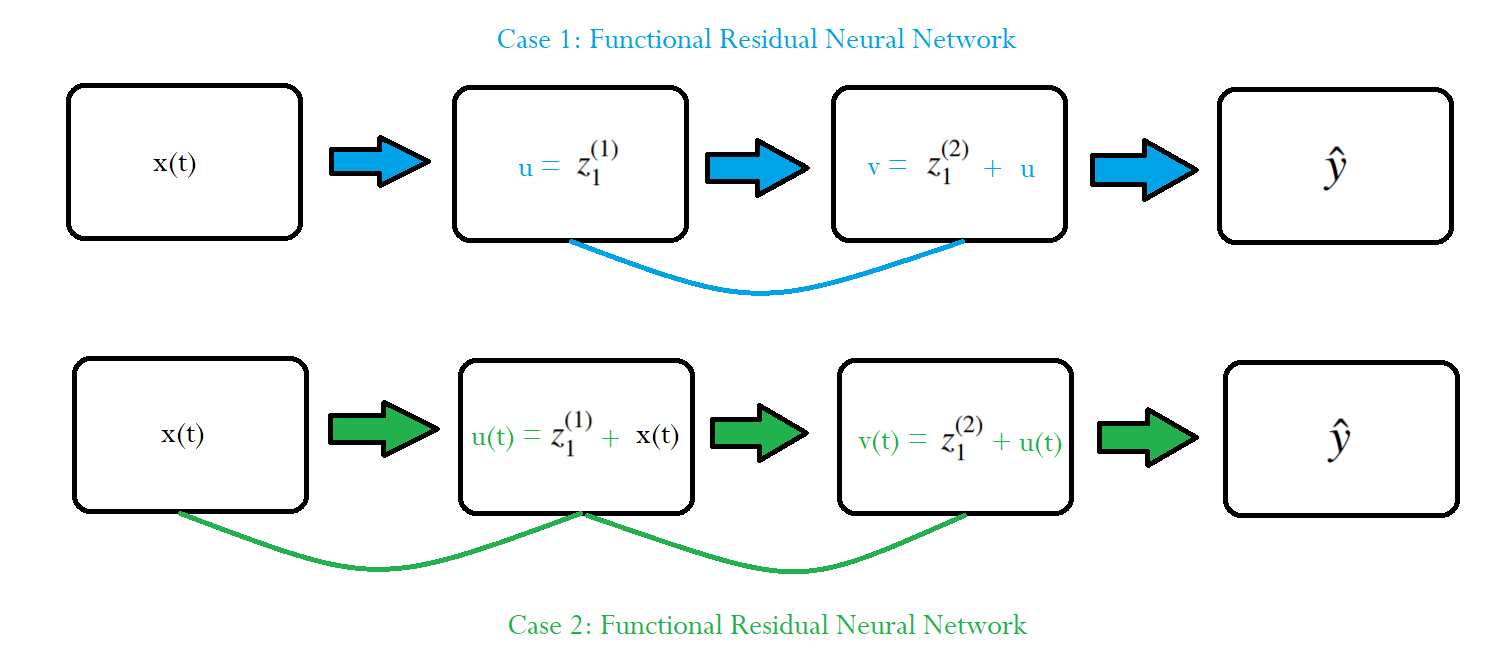
\includegraphics[scale = 0.5]{funcResNN.png}
  \label{fig:flowChartFuncResNN}
  \caption{This is a figure illustrating the basic difference between the two types of functional residual neural networks. Case 1 is when the residual blocks begin after the first hidden layer. The 2$^{nd}$ case is when the user wants the freedom to use the residual blocks anywhere in their network. This illustration is representative of a neural network with two hidden layers and a single neuron in each - ultimately predicting some scalar value, $\hat{y}$}
\end{figure}

\noindent In essence, there are two different forward passes here that we can use and this implies (although, I suppose not necessarily) that there will be two different backpropagation algorithms used.


\subsubsection{Backpropagation: Scalar Response, Functional Covariate(s)}
\label{sec:backpropResFuncNN}

\noindent First, we will consider the backpropagation algorithm for \textit{case 1} as outlined in \hyperref[fig:flowChartFuncResNN]{Figure 9}. This is the simpler case and hence, the problem reduces to an extension of the backpropagation in the feed-forward case. The derivatives will now be taken with respect to both terms that make up each activation where there is a residual block. This is theoretically not \textit{any} different than the previous approach except the form of the function we are taking the derivative of has changed - everything else follows.
\begin{algorithm}[H]
\caption{Backward Pass - Functional Residual Neural Network - \textit{Case 1}}\label{alg:backwardfuncnnRes}
\begin{algorithmic}[1]
\Statex \textbf{Input}: $\Hat{y}, \theta$, $j$. $i = 0$
\Statex \textbf{Output}: Updated values for the set of parameters $\theta$
\State While $j > i$:
\State Select a subset number, $f$ of observations for which the neural network is run - a mini batch
\State Compute the gradient, $\nabla R$ for each observation
\Statex An example of this is given as follows in consideration of the canonical example to make clear the difference between residual and feed-forward neural networks:
\begin{align}
    \dfrac{\partial R}{\partial W_{3}} = -2\cdot(y - \hat{y})\sigma^{'}(t_{3})\cdot z_{1}^{(2)} + \dfrac{\partial z^{(2)}}{\partial w_{3}}
\end{align}
Since now, the additional pass of the previous activation also needs its derivative computed with respect to the parameter being considered ($t_3$ is the linear combination associated with the activation value)
\State Take the average of the corresponding gradient values across all the observations
\State Add the average, weighted by some learning rate $\gamma$ to the current values of the weights: $w_i = w_i + \dfrac{\partial R}{\partial _{w_i}}\cdot\gamma$ where $w_i$ is some parameter of the network, $\hat{y}$
\State $i = i + 1$
\State Go back to 1
\end{algorithmic}
\end{algorithm}
\noindent Consider now, \textit{case 2}. One approach is to take the basis expansion of every single one of the coefficient functions. From here, the problem has been reduced as in \textit{case 1} and we can proceed as per usual. Note however, the computational inefficiency noted earlier - given this inefficiency, we consider an alternative approach using a continuous analogue of the chain rule: \textit{the adjoint method} - however, this will reserved for future work.

\subsubsection{Current Status:}

\noindent The other variations of this type of network, implicated in \hyperref[fig:family]{Figure 1} are still in development.

%\subsubsection{Forward Pass: Functional Response, Scalar Covariate(s)}

%\subsubsection{Backpropagation: Functional Response, Scalar Covariate(s)}

%\subsubsection{Simulation Study: Functional Response, Scalar Covariate(s)}

%\subsubsection{Forward Pass: Functional Response, Functional Covariate(s)}

%\subsubsection{Backpropagation: Functional Response, Functional Covariate(s)}

%\subsubsection{Simulation Study: Functional Response, Functional Covariate(s)}

\subsection{Functional Recurrent Neural Networks}

\subsubsection{Current Status:}

\noindent The variations of this type of network, implicated in \hyperref[fig:family]{Figure 1} are still in development.

%\subsubsection{Simulation Study: Scalar Response, Functional Covariate(s)}

%\subsubsection{Forward Pass: Functional Response, Scalar Covariate(s)}

%\subsubsection{Backpropagation: Functional Response, Scalar Covariate(s)}

%\subsubsection{Simulation Study: Functional Response, Scalar Covariate(s)}

%\subsubsection{Forward Pass: Functional Response, Functional Covariate(s)}

%\subsubsection{Backpropagation: Functional Response, Functional Covariate(s)}

%\subsubsection{Simulation Study: Functional Response, Functional Covariate(s)}

\subsection{Functional Neural Ordinary Differential Equations}

\noindent This network and its variations will be reserved for a future work.

\section{Conclusions \& Future Considerations}

\noindent The advent and rise of neural networks has resulted in enormous breakthroughs in computer vision, classification, and scalar prediction. However, these advantages thus far had been limited to the multivariate space. This paper introduced a family of neural networks that extend into the functional case. 

\noindent In particular, the family of neural networks introduced encompasses feed-forward, residual, and recurrent models; for each of these, three combinations of inputs and outputs were given. Namely, the six possible permutations of functional and scalar responses and covariates were of interest. Algorithms were introduced that detailed the steps required to compute a solution for the network. These algorithms took advantage of Gaussian Quadrature and the usual backpropagation algorithm to compute integral approximations and weight updates for the functional observations (over the relevant time intervals). For the project, this was presented only for feed-forward and residual neural networks of one type. Moreover, an example was provided that showed that the functional neural network outperformed not only functional linear regression but also the classic neural networks with respect to squared error and test predictions. Lastly, it was shown that the usual black-box nature of regular neural networks is somewhat remedied here; in fact, it is possible to extract out interpretable \textit{functions} from these models akin to the coefficient functions in functional linear regressions.

\noindent To extend this project, algorithms will be developed for the other combination of input and output types. Additionally, a promising area of research moving forward could be an expansion into the new world of \textit{Neural Ordinary Differential Equations}. This approach will perhaps allow us to compute derivatives directly of the functions using the adjoint method which isn't a luxury in the discrete case(s) presented here - an introduction in provided in the appendix. There is also potential for the application of classical statistical techniques used for uncertainty calculation; since we have the variation available to us on the $\beta$ coefficient curves for each functional observation, it seems natural that we should be able to extend this to find confidence intervals. Regardless, this is an open area of research with lots of potential for creative extensions.



\newpage
\section{References}
\label{sec:six}
\nocite{ESL, resnetCode}
\nocite{jseam2_2019}
\nocite{rscratch}
\nocite{ode_imp2, odeVid, aisc_2019, reticulate, kaustav1987, drchainsaw_2019, R1, R2, cao}
\printbibliography[heading= none]{}

\section{Acknowledgments}
\label{section:zero}
\noindent A special thank you to Jiguo Cao\footnote{Professor of Statistics, Simon Fraser University}, Lucas Wu\footnote{Department of Statistics \& Actuarial Science, Simon Fraser University}, and Kevin Multani\footnote{Department of Physics, Stanford},  for their contributions to this work.

\newpage
\section{Appendix}
\label{sec:appendix}
\subsection{Functional Data}
\label{sec:functionaldata}

\noindent The functional data analysis introduction here is hardly exhaustive. Curious readers should consult Ramsay and Silverman's \textit{Functional Data Analysis} \cite{fda}.

\subsubsection{Motivation}

\noindent Often, we have repeated measurements of some number of individuals over a time interval, \textbf{T}. Normally, this data would be presented as discrete values however, a lot more can be gleaned from the information available if the discrete data for each subject is treated as a single \textit{functional} observation rather than as a collection of multivariate data. In particular, you may be able to take derivatives to infer how the underlying function changes over time. For example, imagine that you had height data over time for a number of children. Then, finding an underlying function could allow you to understand how growth \textit{accelerates} or slows down at a particular age. 


\subsubsection{Turning Discrete Data into Functional Data}

\noindent Basis functions are used to represent functions. Think of observed discrete data points as single entities. Functional is a reference to the intrinsic nature of the data. Functional data is also observed and recorded as a pair: $(t_j, y_j$) - this can be seen as a snapshot of the function at some time $t$\footnote{Note that time is not the only domain for which functional data can exist, for example, it could also be spatial}. 

\noindent Let $x(t)$ be the functional observation to be estimated. We assume that $x(t)$ has reason to exist in the given context. We also must get $x(t)$ to be smooth as this is what differentiates functional data from multivariate data. It also indicates that derivatives exist. For example, we can estimate the various dynamics: position, velocity, and acceleration if we had functional observations for such data. There is also another important term: signal-to-noise ratio. This is the amount of measurement error to actual usable data. In this section, we explore ways to estimate $x(t)$ using basis systems. 

\noindent In general, we are concerned with a collection or sample of functional data, rather than one single functional observation, $x(t)$. For example, here is what a set of functional observations might look like in matrix form:
\[ x_i = (t_{ij}, y_{ij}) = 
\begin{bmatrix}
    (t_{11}, y_{11}) & (t_{12}, y_{12}) & ... & (t_{1n}, y_{1n}) \\
    ... & ... & ... & ... \\
    ... & ... & ... & ... \\
    ... & ... & ... & ... \\
    (t_{m1}, y_{m1}) & ... & ... & (t_{mn}, y_{mn}) \\
\end{bmatrix}
\]

\noindent Where each row can be thought of as a separate functional observation to be estimated. Note that sometimes the $t$ values might be the same across all discrete data points, hence the notation can be simplified. For the rest of this section, we usually assume that we are dealing with a single $x(t)$ estimation\footnote{However, if the signal-to-noise ratio is low, then using information from other curves might prove fruitful}. 

\noindent There are two basic subsets in which the time component of functional data is distributed: periodically and non-periodically. Examples of periodic data might be the calendar year where $t$ loops around after December. Non-periodic data might be information collected pertaining to hand movements while someone uses a pen. Also, functional data itself could be distributed over multiple domains; for example, the continuum's could be space and time. 

\noindent Since our function fit will not be exact to the discrete data points, the assumption is made that the difference between the function fit and the discrete value is a matter of random error (corresponding to the "roughness" of the data). That is:
\begin{align}
y_j = x(t_j) + \epsilon_j
\end{align}
\noindent Alternatively, we can write this in matrix notation as: \textbf{y = x + e}. We can assume the function values to be fixed effects and therefore, they have 0 variance. This implies that the variance-covariance matrix of \textbf{y} is equivalent to the variance-covariance matrix of the error term denoted as $\sum_e$. The variance of the residuals varies over the argument, $t$\footnote{For example, error in height measurements changes with age}. Consideration also needs to be given to the correlation between neighboring residuals - normally known as the autocorrelation. 

\noindent The resolving power of data is the density of the argument values, $t_j$ relative to the amount of curvature. This is in contrast to just using $n$ as a measure of sparsity in the data set. Essentially, if curvature is high, then more points are required and if curvature is low, then less points are required for accuracy. 

\subsubsection{Basis Functions}

\noindent A basis function system is a set of known functions, $\phi_k$, such that the functions are independent of one another. The main property of such a system is that the set of $K$ functions in the basis is a linear combination that can approximate any function arbitrarily well. For example, the monomial basis system includes the functions: $\{ 1, a, a^2, a^3, ... \}$. Functions are represented as:
\begin{align}
x(t) = &= \sum_{k = 1}^{K}c_k\phi_k(t) \\
&= c_1\phi_1(t) + c_2\phi_2(t) + ... + c_K\phi_K(t) \\
&= c^T\phi
\end{align}
\noindent The dimension of the expansion is $K$. We are essentially representing the infinite-dimensional $x(t)$ in a finite space as this basis. When $K = n$, we get an exact interpolation\footnote{That is: $x(t_j) = y_j$}. With a smaller $K$ and a better choice in basis, we are given the privilege of more degrees of freedom and less computational time. The behavior of the derivative of the estimated fit can be a good measure of what a good basis choice is; a good basis for $x$ might not be a good basis for $Dx$.

\subsubsection{Smoothing Functional Data by Least Squares}

\noindent In the previous section, we discussed how to select a basis depending on the type of data you have however, remember that a functional data object is defined as:
\begin{align}
y_j = \sum_kc_k\phi_k(t_j)
\end{align}
\noindent So how then, do we calculate the coefficient $c_k$? One method to do so is to use the classic ordinary least squares estimation. If we defined $\Phi$ to be the $n$ by $K$ matrix containing our $K$ basis functions each evaluated at the values of $t$, then the estimate for $c_k$ is:

\begin{center}
$\hat{c} = (\Phi^T\Phi)^{-1}\Phi^Ty$
\end{center}

\noindent And therefore, $\hat{y} = \Phi(\Phi^T\Phi)^{-1}\Phi^Ty$. This is called the least squares smoother in the context of functional data analysis. However, the classic model may not always be realistic for the data we have due to autocorrelation and non-stationarity of the residuals. A weighted least squares method may be used alternatively in that case. The estimate then becomes:
\begin{align}
\hat{c} = (\Phi^T\Phi)^{-1}\Phi^TWy
\end{align}
\noindent Where W is a symmetric positive definite matrix. If $\sum_e$ is known then, W = $\sum_e^{-1}$. Note that the coefficient matrix is often called the projection matrix\footnote{Which means the image of y has residuals orthogonal to the fit oof $\hat{y}$} and has the property of being idempotent (that is, if the matrix was defined as $S$, then $S = SS$). 

\noindent Some commentary on least squares degrees of freedom: In most books, the degrees of freedom of a fit is the number of parameters estimated from the data that are required to define the model however, for a smooth fit, the degrees of freedom is defined as the trace of the project matrix, $S$. Turns out that this value is equal to $K$ in the ordinary least squares case. 

\subsubsection{Bias-Variance Trade-Off}

\noindent The higher the number of basis functions chosen, the closer the fit is to the discrete data (implying a lower bias) however, you run the risk of fitting to noise in this case. On the hand, the lower the value of $K$ is, the less accurate your predictions will be and thus, you can expect your fit to be less relevant to the given context (so, lower variance but higher bias).

\noindent We want to minimize the mean squared error which is well defined as:
\begin{align}
MSE[\hat{x}(t)] = bias^2[\hat{x}(t)] + var[\hat{x}(t)]
\end{align}

\subsubsection{Smoothing Functional Data with a Roughness Penalty}

\noindent Basis functions are good approximations if the functions picked have similar characteristics as the underlying data generating process. However, the methods discussed in the previous section have clumsy discontinuity issues with respect to smoothing. The smoothness used with a roughness penalty makes it explicit in the minimization criterion, what it is that is being minimized. 

\noindent Imagine you have a function \textbf{x(t)} to be estimated which is non-periodic. Then, remember there are two competing goals: to have a good fit and to reduce "wigglyness" or roughness. How does one measure roughness? One way is to look at the square of the second derivative at some time, \textit{t}, defined as the curvature. This is a good measure because a straight line is considered to be perfectly smooth and the second derivative of such a curve is 0. Curvature is defined as:
\begin{align}
PEN_m(x) = \int[D^mx(s)]^2 ds
\end{align}
\noindent Incorporating this curvature measure into our least squares minimization criteria yields:
\begin{align}
PENSSE_\lambda(x|y) = [y - x(t)]^TW[y - x(t)]^2 + \lambda PEN_2(x)
\end{align}
\noindent Here, $\lambda$ is a smoothing parameter that measures the trade-off between a good fit and the curvature (or variance) of the data. The larger $\lambda$ is, the more smooth our fit because roughness is being penalized heavier. On the other hand, the smaller $\lambda$ is the, the more closer the fit is (lower bias) to the original data points. When $\lambda$ = 0, we have the weighted least squares case. 

\subsubsection{Functional Linear Models}

\noindent There are three basic types of functional linear models:
\begin{itemize}[label={\ourShadow{$\star$}{black}}] 
    \item Scalar response, functional covariate
    \item Functional response, scalar covariate
    \item Functional response, functional covariate
\end{itemize}
\noindent The focus here will be on the first. The usual functional linear model is notated as follows:
\begin{align}
    E(Y|X) = \alpha_0 + \int_{0}^{T} \beta(t)x_i(t)dt
\end{align}
\noindent Where $\alpha_0$ is the intercept term and you could think of $\beta(t)$ as a function which generates the coefficients associated with the co-variate at any point from 0 to $T$. Also, $x_{i}(t)$ is the $i^{th}$ functional functional observation used to predict the scalar response $y$.

\noindent The next question then is: how do we estimate $\beta(t)$? This is done in the usual way - by minmimizing error. 
\begin{align}
    \beta(t) = argmin\left\{\sum(y_{i} - \alpha_{0} -  \int_{0}^{T} \beta(t)x_i(t)dt)^{2} \right\}
\end{align}
\noindent However, this can result in volatile estimates along with some significant probability of over-fitting. Instead then, a constrained approach is used:
\begin{align}
    PENSSE_{\lambda}(\beta) = argmin\left\{\sum(y_{i} - \alpha_{0} -  \int_{0}^{T} \beta(t)x_i(t)dt)^{2} + \lambda \int[\beta(t)]^{2}dt \right\}
\end{align}
\noindent Note: we still represent $\beta(t)$ in some functional form $\beta(t) = \sum c_i\phi_i(t)$. Now, let $Z_i = [1, \textbf{x}_i]$ and $\textbf{x}_i = \int\Phi(t)x_i(t)dt$. Then, we can rewrite the model as: 
\begin{align}
    \textbf{y} = \textbf{Z} \hspace{0.2em}[\alpha \hspace{0.8em} \textbf{c}]^T + \epsilon
\end{align}
\noindent Essentially then, the vector in the above equation is what we need to estimate. Under the smoothing conditions, the estimate is:
\begin{align}
    [\hat{\alpha} \hspace{0.2em} \hat{c}^{T}]^{T} = (Z^{T}Z + \lambda R_{L})^{-1}Z^{T}\textbf{y}
\end{align}
\noindent And hence, predictions are given by:
\begin{align}
    \hat{\textbf{y}} = \int \hat{\beta}(t)x_i(t)dt =  \textbf{Z} \hspace{0.2em}[\hat{\alpha} \hspace{0.8em} \hat{\textbf{c}}]^T
\end{align}
\noindent Lastly, note that the parameter $\lambda$ can be chosen through some cross-validation technique revolving around mean squared error.


\subsection{Neural Networks}
\label{sec:nn}

\noindent Neural networks have excelled at prediction problems over the last decade. In this section, I highlight the underlying methodology and present a couple of coding examples.

\subsubsection{Forward Pass}

\noindent For simplicity sake, we will first look at a network with just a "singe hidden layer". Consider \hyperref[fig:nn1]{Figure 10} - the \textcolor{cyan}{blue} \textit{"neurons"} contain values of the input data. For example, if the input was an image, then each neuron would hold a value corresponding to the gray scale value of each pixel of the image. This is known as the \textit{activation} value. The \textcolor{red}{red} neurons contained within the second row are referred to as neurons from the \textit{hidden layer}. Each single layer is a non-linear transformation of a linear combination of each activation in the first layer. For example, $z_1$ would be defined as:
\begin{align}
    z^{(1)} = \sigma(\vec{\alpha_{0_{1}}} + \vec{x}\boldsymbol{\alpha^{(1)}})
\end{align}
\noindent Where $\boldsymbol{\alpha^{(1)}}$ and $\vec{\alpha_{0_{1}}}$ is the set of weights and biases\footnote{These are initialized randomly in this simple case} and $\sigma()$ is some \textit{activation function} that transforms the resulting linear combination so that it can provide us with useful numbers (for example, we might want probabilities for a binary response so we could use the sigmoid function\footnote{$\dfrac{1}{1 + e^{-x}}$} when that is the case). Note that the vector $\vec{x}$ corresponds to a single "row" of our data set (or, a single image if that was the data type we were working with) and is therefore a $p$-dimensional vector where $p$ is the number of covariates.

\begin{figure}[h!]
  \centering
  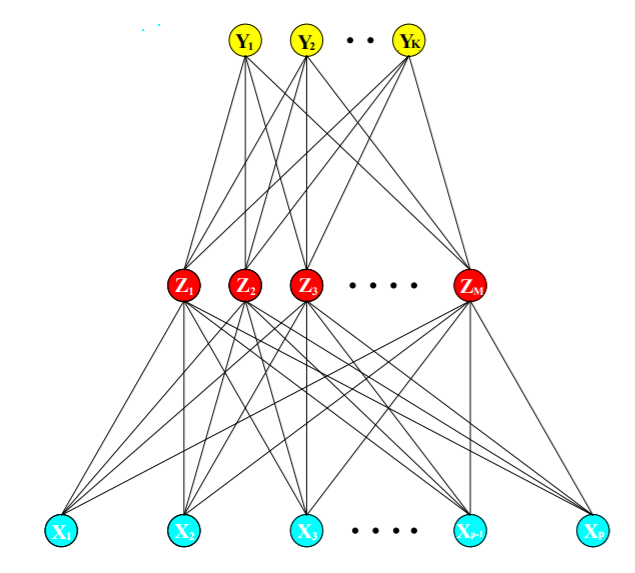
\includegraphics[scale = 0.75]{nn1.png}
  \label{fig:nn1}
  \caption{An overview of a single hidden layer network \cite{ESL}}
\end{figure}

\noindent Once we have the values for the $m$\footnote{The choice of $m$ is left to the user} neurons in the hidden layer, we have another set of activations! Using these, we can move onto the \textcolor{yellow}{final layer}. In the case of image classification, say for the purposes of number recognition, an image might correspond to a single number $y \in \{0, 1, 2, 3, 4, 5, 6, 7, 8, 9\}$. In this case, $K = 10$ and is the number of possibilities for classification. The last transformation assigns a probability to each of the $K$ classes effectively providing a likelihood that your observation (in our example, the single image) belongs to each of them, respectively. Often, the softmax function:
\begin{align}
    g_{k}(T) = \dfrac{e^{T_k}}{\sum_{i = 1}^{K}e^{T_i}}
\end{align}
\noindent is used as it allows probability specification for a number of classes\footnote{In fact, letting $k \in \{0, 1\}$ returns the famous logistic transformation}. Here, there are $k$ sets of $T$ values and these are all linear combinations moving from the hidden layer to the output layer. You can imagine that this could be generalized to $n$ number of hidden layers with some choice of $m$ neurons in each of them resulting in a myriad of parameters to be estimated!

\subsubsection{Backpropogation}

\noindent The "learning" of this approach takes place in a process called \textit{backpropogation} - this is just jargon for gradient descent. In order to do so, we must first define a loss function. This function is some measure of the aggregated residual between our prediction and the true value. One approach is to use squared-error:
\begin{align}
    R(\theta) = \sum_{k = 1}^{K}\sum_{i = 1}^{N}(y_{ik} - f_{k}(x_i))^2
\end{align}
\noindent This function is a sum of the difference between the prediction for every observation for every output. For example, the outer sum would be of the difference between the predicted probability of an image belonging to a particular class, over all classes and the inner sum would aggregate over every image (or observation) you have\footnote{There are a plethora of loss functions to pick from; for example, cross-entropy and log-loss}. 

\noindent Now that we have a measure of error, we can look to minimize it! This function takes in $(p + 1)\cdot M\cdot (M + 1)\cdot K$ parameters\footnote{The set $\theta$ encompasses these parameters} so we will have a very high dimensional gradient. This results in an inordinate amount of peaks and valleys on the optimization landscape. It is also very likely that the global minimizer of $R(\theta)$ will overfit the data so any local minimizer may serve us better; in fact, we will take small steps towards the optimum specified by a "learning rate", $\gamma$.

\noindent For simplicity sake, we consider a network with a single neuron in its 2 hidden layers and only look at a 1-dimensional observation \cite{3blue1brown_2017}.

\begin{figure}[h!]
  \centering
  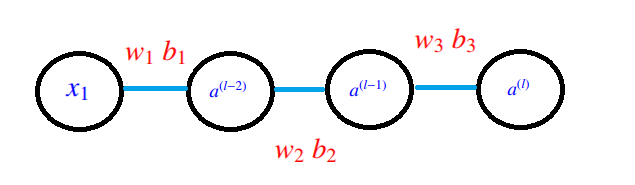
\includegraphics[scale = 0.7]{schema.png}
  \label{fig:schema}
  \caption{Schematic representing toy example}
\end{figure}

\noindent Then, the cost function, $R$ will have 6 parameters outlined in \textcolor{red}{red} in \hyperref[fig:schema]{Figure 11}. Using (3), we see that in this simple case, the cost function reduces to $R_{1} = (z^{(l)} - y)^2$ where $a^{(l)}$ is the activation in the final layer\footnote{Let $l$ be indicative of the last layer i.e. $w_3 = w^{(1)}$ and $w_2 = w^{(l - 1)}$} defined as: $a^{(l)} = \sigma(w^{(l)}a^{(l - 1)} + b^{(l)})$. For convenience, define $w^{(l)}a^{(l - 1)} + b^{(l)}$ as $u^{(l)}$. Remember, we want to minimize the cost function; we can note that a change in the weight $w^{(l)}$ causes some change to the cost function, $R_{1}$ - we want to know this change: $\dfrac{\partial R_1}{\partial w^{(l)}}$ as our goal is to minimize this. Using chain rule, we can observe that this derivative can be broken down to a number of sub-derivatives:
\begin{align}
    \dfrac{\partial R_1}{\partial w^{(l)}} &= \dfrac{\partial u^{(l)}}{\partial w^{(l)}}\cdot\dfrac{\partial a^{(l)}}{\partial z^{(l)}}\cdot\dfrac{\partial R_{1}}{\partial a^{(l)}}\\ \vspace{3em}
    &= a^{(l - 1)}\cdot\sigma^{'}(z^{(l)})\cdot2\cdot(a^{(l)} - y)
\end{align}
\noindent We want to find the roots of this derivative but, not ONLY this derivative. First, we note that (3) is defined for every observation: 
\begin{align}
    \dfrac{\partial R}{\partial w^{(l)}} = \dfrac{1}{n}\sum_{i = 0}^{n - 1}\dfrac{\partial R_i}{\partial w^{(l)}}
\end{align}
\noindent And note that (6) is only one of the 6 derivatives making up the gradient of the cost function:
\[\nabla R = \Bigg( \begin{array}{cc}

\dfrac{\partial R}{\partial w^{(l)}} \ \ \
\dfrac{\partial R}{\partial w^{(l - 1)}} \ \ \ 
\dfrac{\partial R}{\partial w^{(l - 2)}} \ \ \ 
\dfrac{\partial R}{\partial b^{(l)}} \ \ \
\dfrac{\partial R}{\partial b^{(l - 1)}} \ \ \
\dfrac{\partial R}{\partial b^{(l - 2)}}
\end{array} \Bigg)^{T} = \textbf{$\vec{0}$}\] \\
\noindent The parameter values that satisfy the above equation are the changes we need to make to the current weights. The change is done proportional to the aforementioned learning rate, $\gamma$. This approach is taken for computational efficiency - finding the full gradients is nearly impossible so the optimal values are found in \textit{mini batches}; these are subsets of observations for which the optimization takes place as opposed to the entire data set. This approach is also known as \textit{stochastic gradient descent}. The process repeats for some number of \textit{epochs}\footnote{A single epoch is one full forward and backward pass for every observation in your data set}. 

\noindent In summary, you begin with a set of weights, train the model, and get predictions. You run these predictions through a loss function and attempt to minimize it by updating the parameters of the function according to the gradient. You do this at some learning rate and the evaluations are done on subsets of data (mini batches) for some number of iterations.

\noindent In this \hyperref[sec:resnn]{subsection}, a primer is provided on \textit{residual neural networks} - a clever extension that circumvented the vanishing gradient problem.


\subsubsection{Data Description}

\noindent The data set is taken from a 2017 Kaggle competition \cite{iceberg} in which participants were asked to classify satellite images as either icebergs or ships. There are two variables corresponding to the pixel values of the images ($x, y$ coordinates) and a unique \textit{ID} variable which corresponds to the $i$ index in the theory above (observation number). There's a final binary (output) variable which classifies the image as an iceberg (or not). In \hyperref[fig:iceberg_images]{Figure 12}, some of the images are visualized.

\begin{figure}[h!]
\centering
  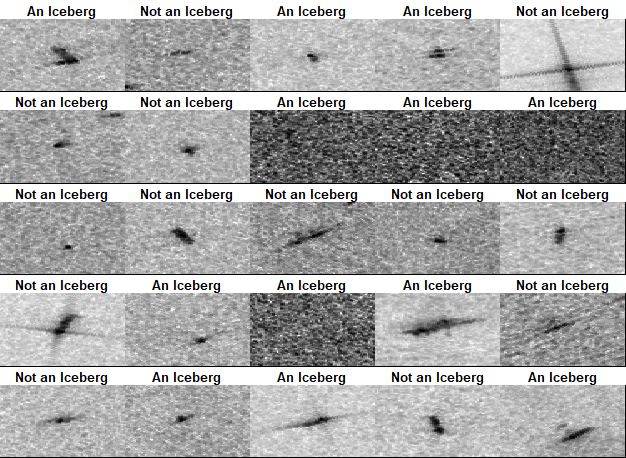
\includegraphics[scale = 0.55]{iceberg_img.png}
  \label{fig:iceberg_images}
  \caption{A snapshot of the grayscale iceberg/not iceberg images}
\end{figure}

\subsubsection{Model Specifics}

\noindent The model was trained on 1300 images and used to predict 304 \cite{allaire}. The activation function used in the 4 \textit{dense} hidden layers was \textit{relu}\footnote{$\sigma(z) = max\{0, z\}$} and the sigmoid function was used for the output. The optimization landscape was explored by \textit{stochastic gradient descent} (sgd) and loss was characterized by \textit{binary cross-entropy}.

\subsubsection{Performance}

\noindent The model performed with exceptional mediocrity after being run through 150 epochs. \hyperref[fig:lossNN]{Figure 13} provides the loss results for the model as it worked its way through the epochs. The final accuracy on the test images was: 54\%.

\begin{figure}[h!]
  \centering
  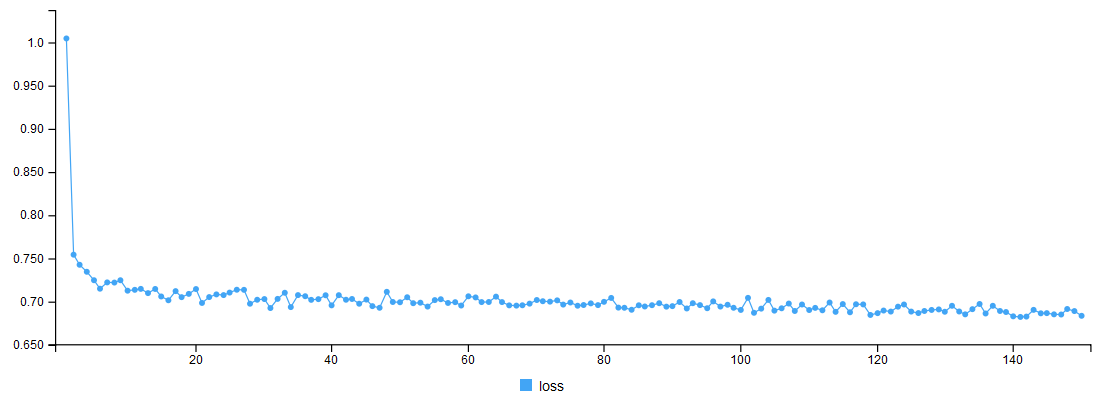
\includegraphics[scale = 0.4]{loss_plot3.png}
  \label{fig:lossNN}
  \caption{Accuracy results for neural network model}
\end{figure}

\subsubsection{An Example from Scratch}

\noindent A model was trained in R which was used to predict a binary response from normally generated data. The response, $y$, was 1 if the randomly generated Gaussian data point was between -0.5 and 0.5 and 0 otherwise. The model was set to predict all 0's in the beginning and had an accuracy of 0.64. After training the model for 50 epochs, the  model had an accuracy of 1. The MSE loss plot is given in \hyperref[fig:scratchNN]{Figure 14}:

\begin{figure}[h!]
  \centering
  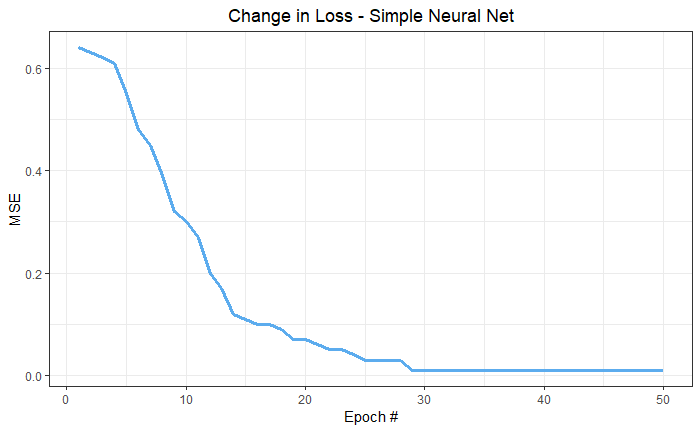
\includegraphics[scale = 0.7]{NN_scratch_loss2.png}
  \label{fig:scratchNN}
  \caption{Loss results for hand-coded neural network}
\end{figure}


\subsection{Residual Neural Networks}
\label{sec:resnn}
\noindent In this section, I introduce an extension to deep neural networks developed by researchers at Microsoft \cite{resnet}. 

\subsubsection{Residual Blocks}

\noindent A common problem with recurrent (plain) neural networks is their inability to be trained on a large number of hidden layers. This problem arises due to vanishing (and exploding) gradients. A vanishing gradient occurs for weights and biases earlier in the network. Recall that, during backpropagation, we use chain rule to find gradient values and that, the further back we are, the more terms there are that are used to compute the gradient. Since there are more terms, their exists a higher probability that some of those terms will be small and hence, due to the multiplicative nature of the chain rule, there becomes a tendency for those earlier weights to hardly even move during the update portion of the iteration\footnote{The update is: $w_{i} = w_{i - 1} - \gamma \cdot \dfrac{\delta R}{\delta w_{i - 1}}$. That is to say, the second term in this equation can become very small} \cite{deep}.

\begin{figure}[h!]
  \centering
  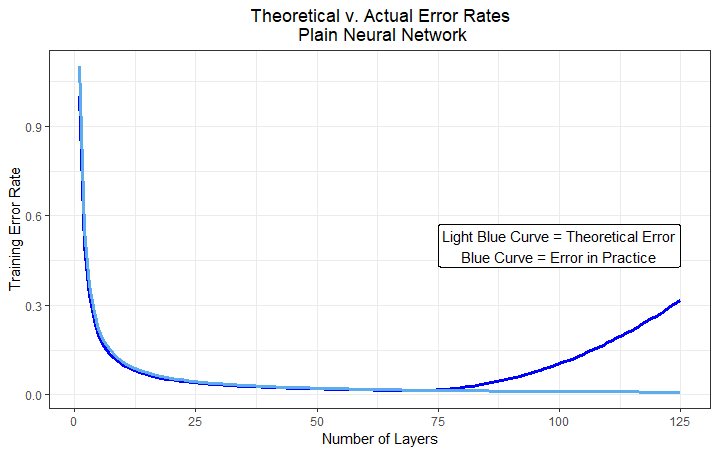
\includegraphics[scale = 0.5]{error_plot2.png}
  \label{fig:error_theory}
  \caption{An overview of the training set error rates for recurrent (plain) neural networks. The vanishing gradient problem is theorized to be responsible for the \textcolor{blue}{blue} curve}
\end{figure}

\noindent A solution to this problem comes in the form of \textit{residual blocks}. These are modifications to the linear part of the neural network in between layers. Consider an activation in classic neural networks:
\begin{align}
    z^{(1)} = \sigma(\vec{\alpha_{0_{1}}} + \vec{x}\boldsymbol{\alpha^{(1)}})
\end{align}
\noindent Letting $z^{(2)}$ and $z^{(3)}$ be the activations in the second and third layer\footnote{These are single dimensional i.e. only a single neuron in each layer. This generalizes easily an $m$-dimensional case where these would be vectors instead}. Then, normally, we would have the following:
\begin{align}
    z^{(1)} &= \sigma(\vec{\alpha_{0_{1}}} + \vec{x}\boldsymbol{\alpha^{(1)}})\\
    z^{(2)} &= \sigma(\vec{\alpha_{0_{2}}} + z^{(1)}\boldsymbol{\alpha^{(2)}})\\
    z^{(3)} &= \sigma(\vec{\alpha_{0_{3}}} + z^{(2)}\boldsymbol{\alpha^{(3)}})
\end{align}
\noindent However, in a residual block we adjust say, $z_3$ so that we get:
\begin{align}
    z^{(3)} &= \sigma(\vec{\alpha_{0_{3}}} + z^{(2)}\boldsymbol{\alpha^{(3)}}) + z^{(2)}
\end{align}
\noindent The key insight here is that as the weights $\boldsymbol{\alpha^{(3)}}$ and the bias $\vec{\alpha_{0_{3}}}$ vanish, the input into the activation function tends toward the identity transformation rather than 0. This means that, instead of having a degradation in learning as we increase the number of layers, the neural network will instead have, at \textit{worst}, an identity transformation layer to layer (that is, the activation function will just take you back to the activation value of the $((i - 2) + 1)^{th}$ layer and allow the optimization to flourish in other elements of the gradient that are not (yet) experiencing the problem.

\begin{figure}[h!]
  \centering
  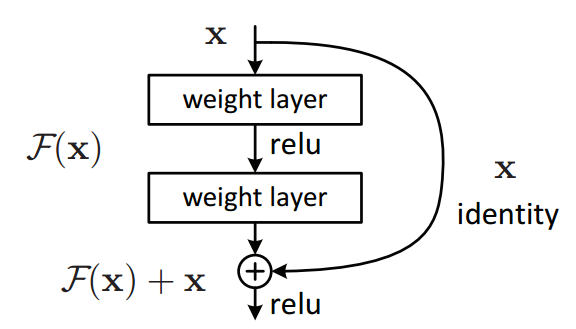
\includegraphics[scale = 0.6]{block.png}
  \label{fig:block}
  \caption{A residual block. The $F(x)$ here is analogous to the $z^{(3)}$ in the notation used here. \cite{res1}}
\end{figure}

\noindent The algorithm for backpropagation remains the same. The additional derivative is computed with respect to the added term but the overall process follows the same logic.

\subsubsection{Results}

\noindent The titanic data set was used once again here for the implementation. The residual blocks were used in conjunction with a convolutional neural network (CNN)\footnote{This choice was made due to the nature of the data} (as opposed to an addition to recurrent neural networks) \cite{resnetCode}. 

\noindent The model used the same number of epochs as the previous neural network and was trained on the same number of images (1300). Batch normalization was applied along with a number of other sub-layers relevant to a convolutional neural network. In \hyperref[fig:acc_resnn]{Figure 17}, we can see the relative superiority of this approach:

\begin{figure}[h!]
  \centering
  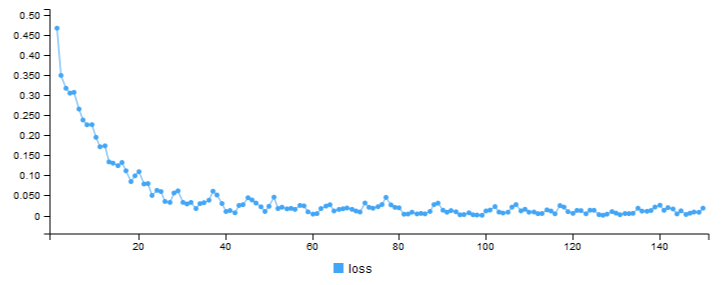
\includegraphics[scale = 0.6]{accuracy_res3.png}
  \label{fig:acc_resnn}
  \caption{Accuracy results for the CNN with residual blocks.}
\end{figure}

\noindent The prediction accuracy for this model on the same set of images was over 87\% using mean squared error as the measure.


\subsection{Differential Equations Primer}
\label{sec:de}

\noindent Discussion in this section will be limited to first order ordinary differential equations. The purpose is to instill enough understanding so that their relevance in \hyperref[sec:neuralODE]{6.6.1} is apparent and clear.

\subsubsection{General Methodology}

\noindent Generally, a differential equation relates the values of some function to the values of its derivatives. A first order differential equation is limited to the relationship between a single derivative of a single variable. They are of the form:
\begin{align}
    \dfrac{dy}{dx} = f(x, y)
\end{align}
\noindent The function $f(x, y)$ is any of the set of functions which is defined for $x$ (the independent variable) and $y$ (the dependent variable). Accompanying the equation is usually an initial condition which defines the behaviour of the function at some point, $x_0$\footnote{The value here is sometimes apparent from the context; for example, consider half-life models in which you know the amount present at time, $t = 0$}. It is sometimes possible to find analytic solutions to differential equations provided they are of a particular form, for example:
\begin{align}
    g(y)\dfrac{dy}{dx} = f(x),\hspace{1em} y(x_0) = y_0
\end{align}
\noindent But, in general, differential equations are solved numerically\footnote{The equation in (6) is known as a separable differential equation because you can split the $f(x, y)$ in (5) into two separate functions}. A method falling under the umbrella of numeric methods is presented in the next sub-section. 

\noindent Let's consider the following ODE:
\begin{align}
    \dfrac{dy}{dx} + \dfrac{y}{2} = \dfrac{3}{2}, \hspace{1em} y(0) = 2
\end{align}
\noindent This differential equation can be solved analytically as follows:
\begin{align}
    \dfrac{dy}{3 - y} & = \dfrac{dx}{2}\\
    \int_{2}^{y}\dfrac{dy}{3 - y} & = \dfrac{1}{2}\int_{0}^{x}dx\\
    \ln{(3 - y)} & = -\dfrac{1}{2}\\
    3 - y & = \exp\{-\dfrac{x}{2}\}\\
    y & = 3 - \exp\{-\dfrac{x}{2}\}
\end{align}
\noindent The solution of the differential equation depends on the initial conditions provided however, the critical points of the function will be clear in any of them. In the above example, when $y = 3$, the derivative is 0 and hence we would expect a horizontal asymptote for any provided initial condition at this value. This behaviour is presented in \hyperref[fig:solutionsCurve]{Figure 18}.


\begin{figure}[h!]
  \centering
  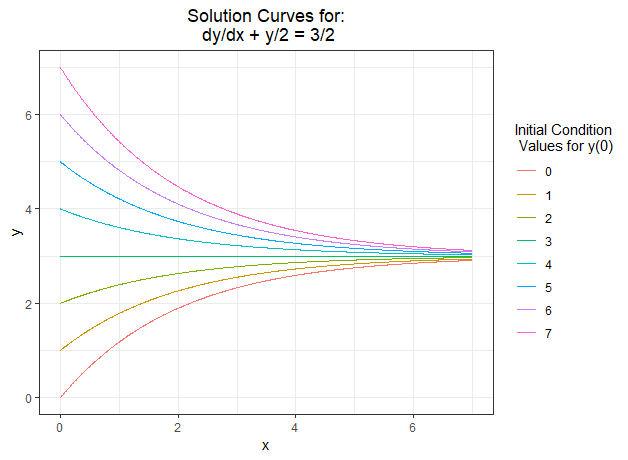
\includegraphics[scale = 0.7]{solution_curves.png}
  \label{fig:solutionsCurve}
  \caption{Solution curves for the ODE given in (7). The particular initial condition that solved for is given by the \textcolor{darkseagreen}{sea green} curve}
\end{figure}

\noindent Another important visualization tool for differential equations is the phase portrait. The phase portrait allows us to discern important information about the original function, $f(x)$ without actually solving the differential equation. The phase portrait involves computing the roots of the function (the 0's of the derivative) and plotting the behaviour of the derivative for various values of the dependent variable, $y$. Consider the following differential equation \cite{de}:
\begin{align}
    \dfrac{dy}{dt} = r(1 - \dfrac{y}{K})y
\end{align}
\noindent Where $K = \dfrac{r}{a}$ and $r$ is known as an 'intrinsic growth rate'\footnote{This equation is an extension on the exponential growth function and is commonly referred to as the Verhulst or logistic equation}. The first step in identifying the phase portrait is to find the 0's; in this case, if we let $y = f(x) = \{0\cap K\}$, then the value of $\dfrac{dy}{dt}$ in (13) is 0 - these are known as the \textbf{equilibrium solutions}. This is when there is no change in the \textit{variation} of $y$ as $t$ changes. From there, we can observe the behaviour of the derivative around these equilibrium points. 

\begin{figure}[h!]
  \centering
  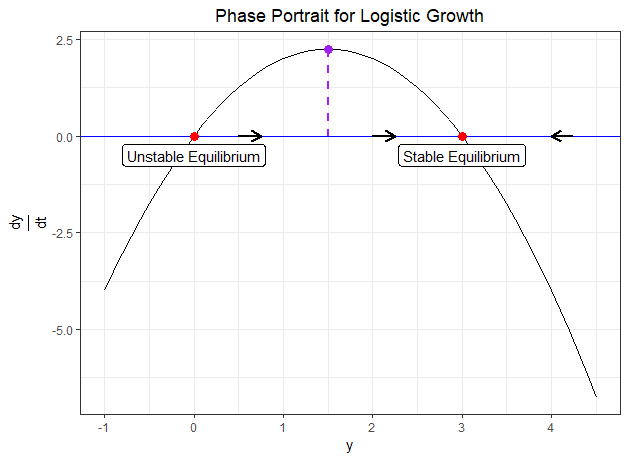
\includegraphics[scale = 0.6]{phasePortrait.png}
  \label{fig:phasePortrait}
  \caption{A phase portrait for the Verhulst Equation defined in (13)}
\end{figure}

\noindent In \hyperref[fig:phasePortrait]{Figure 19}, the arrows point to the right for positive derivative values and to the left otherwise. You can imagine these arrows as directions for convergence. The \textbf{stable equilibrium} is some value that the system being modelled tends to (also known as a saturation level). Intuitively, imagine you were modelling population growth; then, you would expect quicker growth the greater the population size however, at some point resources become limited. This results in a decrease (or stabilization) of the population at some level which, in \hyperref[fig:phasePortrait]{Figure 19}, is the second equilibrium point. The unstable equilibrium in this example, occurs when the population is 0 - we expect no growth if no one is around however, as soon as it is possible to move away from this position, we tend to do so.

\subsubsection{A Numeric Approximation: Euler Method}

\noindent In the previous section, I introduced differential equations, an example of an analytic solution, and visualization tool to glean information about the function $y(x)$ without actually solving the equation; here, I introduce a numerical approach to solving differential equations: Euler method\footnote{This approach is a specification of a more general approach known as Runge-Kutta} 

\noindent Euler's method is an iterative approach that, for some change in $x$, provides an estimate of the function, $f(x)$ using the derivative in the interval, $\Delta (x)$. In order to make this more concrete, consider the differential equation \cite{euler}:
\begin{align}
    \dfrac{dy}{dx} = y, \hspace{1em} y(0) = 1
\end{align}
\noindent The solution, $f(x)$ to this equation is $y = \exp\{x\}$. However, let's assume that we didn't have the means to find the analytic solution and instead, use Euler's method to approximate $f(x)$. Let $\Delta (x) = 1$ be the iterative interval and consider $x = [0, 4]$. At $x = 0$, we have $y = 1$. The derivative at this point is also 0. Then, using the iterative process: $y_{i + 1} = y_{i} + \Delta(x)\dfrac{dy}{dx}$, we see that $y_{1} = 1 + 1\cdot0$ and, redoing this process, we get the following:

\begin{center}
 \begin{tabular}{||c c c c||} 
 \hline
 Iteration & $x$ & $y$ & $\dfrac{dy}{dx}$ \\ [0.5ex] 
 \hline\hline
 0 & 0 & 1 & 1 \\ 
 \hline
 1 & 1 & 2 & 2 \\
 \hline
 2 & 2 & 4 & 4 \\
 \hline
 3 & 3 & 8 & 8 \\
 \hline
 4 & 4 & 16 & 16 \\ 
 \hline
\end{tabular}
\end{center}

\noindent Essentially, we are figuring out the tangent lines for intervals and connecting them - this is our approximation! Note that, as $\Delta(x) \rightarrow{0}$, our approximation approaches the exact solution. A visualization is provided in \hyperref[fig:euler]{Figure 20}.

\begin{figure}[h!]
  \centering
  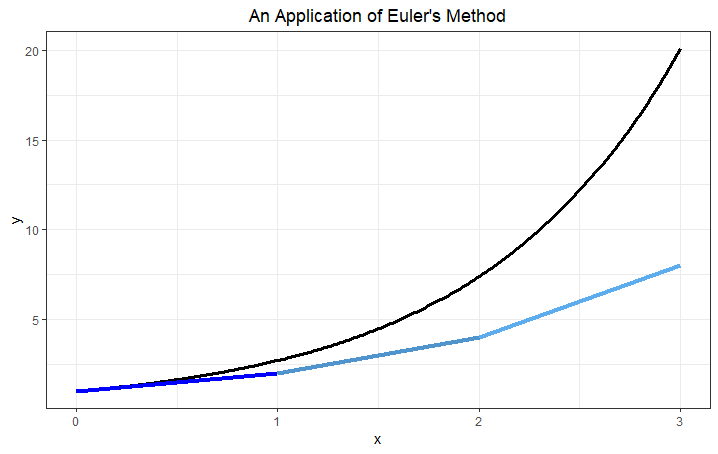
\includegraphics[scale = 0.55]{euler2.png}
  \label{fig:euler}
  \caption{Euler method for the differential equation in (31). The colored segments represent the Euler approximation with a step size of 1. The black curve is the true function: $y = \exp\{x\}$}
\end{figure}

\noindent This brings an end to the primer. The approach in Euler's method is particularly important when comparing ResNets to NeuralODEs in the next section!


\subsection{Residual Networks \& Euler's Method}
\label{sec:resnnEuler}

\noindent Consider again the general transformation performed in ResNets\footnote{In the main section, $z^{(1)} = a_1$} \cite{rajat}:
\begin{align}
    a_1 &= f_{0}(x) + x\\
    a_2 &= f_{1}(a_{1}) + a_{1}\\
    a_3 &= f_{2}(a_{2}) + a_{2}
\end{align}
\noindent Rearranging these, we can observe that this, is almost exactly the form of Euler's method! Letting $a(t = 0) = x$,
\begin{align}
    a(1) - a(0) &= f(a(0), t = 0)\\
    a(2) - a(1) &= f(a(1), t = 1)\\
    ...
\end{align}
\noindent Recall that Euler's method is a descritization dependent on the step size, $\Delta h$. In essence, the key insight of the ResNets approach is characterized by a rearranging of Euler's method. If that is the case, then we are essentially solving a differential equation. A Neural ODE takes another step backwards in the process by appealing to the fundamental equation underlying the neural net rather than looking at the intermediary step that ResNets do.

\subsection{Neural Ordinary Differential Equations}
\label{sec:neuralODE}
\subsubsection{An Overview}

\noindent The main idea underlying the use of differential equations is that they require a fewer number of parameters which contributes to efficiency. To see why, consider a simple linear regression problem where the goal is to estimate optimal values of $a$ and $b$ for $f(x) = ax + b$. Observe that we make an implicit assumption here - the function $f(x)$ is differentiable and so, we can find $f(x)$ directly or we can estimate its derivative, $f'(x)$. The derivative of $f(x)$ is $a$; in the differential equation approach, we only have one parameter to estimate! And, in fact, differential-equation solver approaches don't provide analytic forms of $f(x)$ but rather, numerical values that are dependent on the initial inputs (the data) thus, eliminating the need to ever find $b$ explicitly. 

\noindent Remember that a neural network, more than anything else, is a high dimensional function, $f(\vec{x}; \theta)$ where $\theta$ is the set of weights and biases. Instead of estimating this function, we can model the derivative instead - i.e. the change in the function from layer to layer. Consider some vector \cite{underODE2} of hidden activations\footnote{Moving forward, we will consider the depth (or the hidden layer we are at) by $t$} \footnote{Here, I am going to let the subscript represent where in the network the activations are at}:
\begin{align}
    z_{t + 1} = f(z_{t}, \theta_{t})
\end{align}
\noindent More importantly, in the case of residual networks, the functional form becomes:
\begin{align}
    z_{t + 1} = z_{t} + f(z_{t}, \theta_{t})
\end{align}
\noindent An important insight is the striking resemblance of (13) to Euler's method \footnote{The appendix provides more details} and, recall that Euler's method is a discretization of a continuous relationship between $x$ and $y$ (inputs and outputs). A neural network then, similarly, is also a discretization characterized by the hidden layers. ResNets, while discrete, effectively work as ODE solvers by measuring the rate of differnce in their hidden layers. Let $t$, the depth, go to infinite - then the entire set of layers of a neural network can be written as a differential equation:
\begin{align}
    \frac{\partial z}{\partial t} = f(z(t), t; \theta)
\end{align}
\noindent Intuitively, we have taken a step back in the ODE solving process to where we now have an option on which direction to go to solve the problem. In ResNets, Euler's method is the specified direction however, we aren't limited to that approach here and could use more sophisticated and efficient estimators. The authors use a "black-box differential equation solver".

\noindent The trajectory of Euler's method attempts to model the dynamic of the output over the continuum, $x$; analogously, the hidden layers in a neural network represent the dynamics of the hidden activations with respect to the depth of the network. The limit allows us to smooth out this trajectory so that we can evaluate a hidden activation at any depth $\in \mathbf{R}$. Note that the differential equation trajectories will differ depending on the inputs (think of these as initial conditions). In \hyperref[fig:comp_plot]{Figure 21}, I present one such trajectory\footnote{It's the plot on the right hand side}.

\noindent One advantage of such an approach is that there is a constant memory cost with respect to depth. Recall that derivatives in earlier hidden layers would require more operations in the backpropagation process but this is not the case here. This model also has much less parameters than networks with residual blocks and can be computed efficiently by ODE solvers. There is also an advantage associated with irregular time-series model that classic neural networks had trouble dealing with.

\begin{figure}[h!]
  \centering
  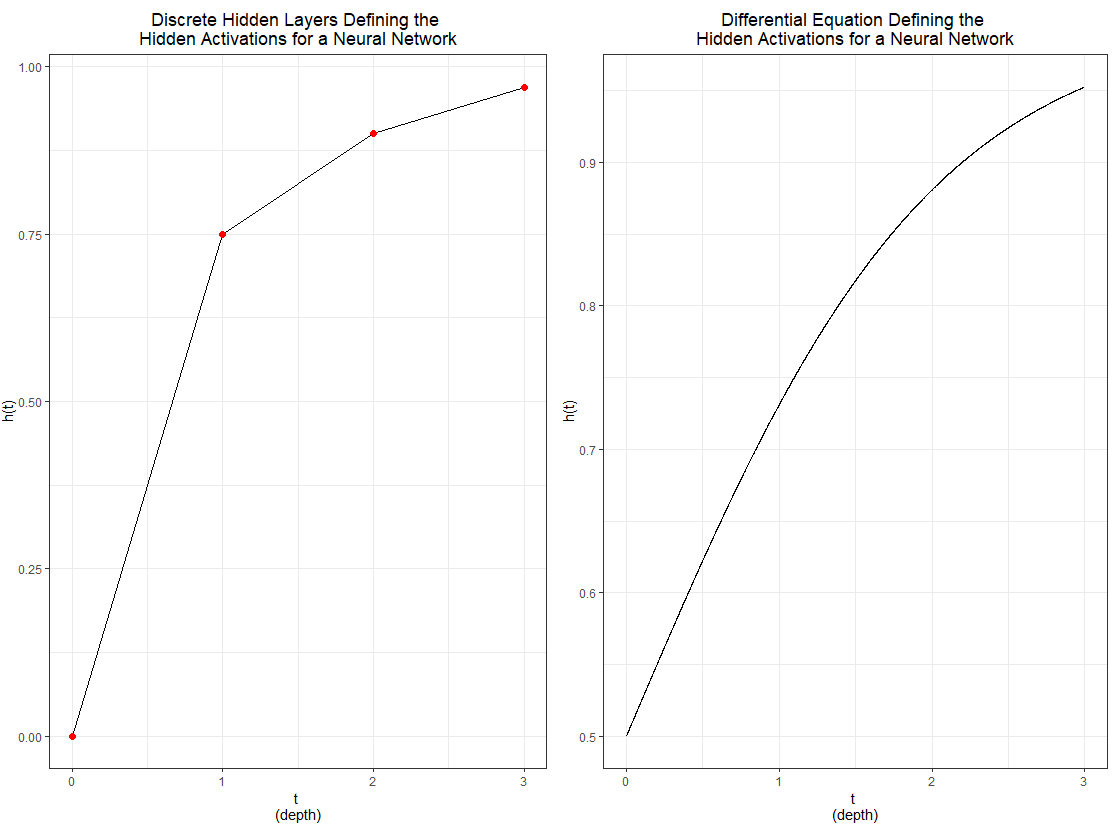
\includegraphics[scale = 0.55]{comp_plot.png}
  \label{fig:comp_plot}
  \caption{Trajectory comparisons of the two hidden state approaches. Note that the \textcolor{red}{red} dots in the left plot are the only evaluations we can do with classic neural networks whereas the dynamics are modeled at any depth in the NeuralODE approach}
\end{figure}

\noindent The hidden state is evaluated by the following integral:
\begin{align}
    z(t) = \int f(t, h(t), \theta_{t}) dt
\end{align}
\noindent Where $\theta_{t}$ is the set of parameters at some layer, $t$. Lastly, note that the initial conditions (that is, at $t_{0}$) are given by the observations, $\vec{x}$ with the output being evaluated at some $t_{j}$ where $j$ is the + 1 iteration from the last hidden state. Deciding on $t_{0}$ and $t_{j}$ is a problem left best to the optimization process; therefore, the final predictions can be summarized as \cite{underODE1}:
\begin{align}
    \hat{y} = z(t_{j}) = ODESolve(z(t_{0}, t_{1}, \theta, f))
\end{align} 
\subsubsection{Backpropagation}

\noindent Now that we have a functional form of the hidden states, we can begin to formulate the backpropagation process. As before, we begin with some (general) loss function:
\begin{align}
    R(t_{0}, t_{1}, \theta_{t}) = R(ODESolve(z(t_{0}, t_{0}, t_{1}, \theta, f)))
\end{align}
\noindent Beginning with the final hidden state, we can compute the gradient: $\dfrac{\partial R}{\partial z(t)}$. We implement the chain rule here because the hidden states themselves are dependent on $t$ - essentially, we are working backwards along the path taken to get to the output, $z(t_{j})$. In the paper, they use the adjoint method \cite{adjoint}. This is a numerical technique used to compute derivatives. An adjoint state is defined as:
\begin{align}
    a(t) = -\dfrac{\partial R}{\partial z(t)}
\end{align}
\noindent This is the change in the loss at any point $t$ in the hidden state interval. Note that the loss function and the neural network are differentiable. We observe then that:
\begin{align}
    \dfrac{\partial a(t)}{\partial t} = -a(t)\dfrac{\partial f(t, z(t), \theta_{t})}{\partial z(t)}
\end{align}
\noindent Which we note is also a differential equation. Using the Fundamental Theorem of Calculus, we can integrate both sides to find a solution for $a(t)$ and, recalling (18), we derive:
\begin{align}
    \dfrac{\partial R}{\partial h(t)} = -a(T) = \int a(t)^{T}\dfrac{\partial f(t, z(t), \theta_{t})}{\delta z(t)} dt
\end{align}
\noindent And finally, we can solve this integral with the black-box ODE solve that was alluded to earlier. Computing this integral from $t{1}$ to $t_{0}$\footnote{Remember, this is a reverse traversal of the hidden states}, we can get the gradient at $t_{0}$. Lastly, the $\theta$ gradient is computed by:
\begin{align}
    \dfrac{\partial R}{\partial z(t)} = \int_{t_1}^{t_0} a(t)^{T}\dfrac{\partial f(t, z(t), \theta_{t})}{\partial \theta} dt
\end{align}
\noindent All of these derivatives can be computed simultaneously as the results do not depend on one another; this parallelization leads to computational efficiency. 


%\begin{figure}[h]
%  \centering
%  \fbox{\rule[-.5cm]{0cm}{4cm} \rule[-.5cm]{4cm}{0cm}}
%  \caption{Sample figure caption.}
%\end{figure}



\end{document}
